\documentclass[11pt,a4paper]{article}

% ---------- Packages ----------
\usepackage[utf8]{inputenc}
\usepackage[T1]{fontenc}
\usepackage{lmodern}
\usepackage[margin=1in]{geometry}

\usepackage{amsmath,amssymb,amsfonts}
\usepackage{graphicx}
\usepackage{booktabs}
\usepackage{siunitx}
\usepackage{xcolor}
\usepackage{authblk}
\usepackage{float}

\usepackage[
  backend=biber,
  style=numeric,
  sorting=none,
  giveninits=true
]{biblatex}
\addbibresource{references.bib}

\usepackage[hidelinks]{hyperref}
\usepackage[capitalise]{cleveref}

% ---------- Title ----------
\title{Learning ATLAS Charge Misidentification Probabilities in Charged Particle Pair Production}

\author[1]{Jeremy J. H. Wilkinson}
\author[1]{Christopher Lester}
\author[1]{Alba Burgos Mondéjar}
\affil[1]{Cambridge University}


\date{\today}

\begin{document}

\maketitle

\begin{abstract}
This paper presents a continuous framework for learning charge-misidentification (QmisID)
probabilities in charged particle pair production. 
As a proof-of-principle, the method is applied to the two-lepton same-charge (2LSC)
channel of the non-resonant di-Higgs analysis. Here an algorithm is setup to
learn the charge-misidentification rate by comparing the kinematic distributions of same-
sign and opposite-sign di-electron events near the Z → e+e− peak, where Standard
Model signatures are dominant. Whereas the state-of-the-art likelihood-based method
uses a coarse 3 × 4 binning, the new method introduced models the charge-misidentification probability as
a continuous function of charged particle kinematics. This refined granularity provides
detector-response information that was previously inaccessible and enables a differential
description of QmisID effects. 
The results showcase how constrained classification, naturally accommodated in machine-
learning platforms, can be used as an instrument for extracting rich detector-level re-
sponse functions. This points toward a new paradigm for precision background estimation
in high-energy physics, with broader implications for current and future LHC analyses.
\end{abstract}

\section{QmisID: Charge Misidentification}

This paper is geared towards the goal of learning particle-level detector response functions that are fully differential. These encompass both continuous functions (i.e. resolution effects) as well as discrete functions. 
Here we focus on the second task: learning to predict whether a particle produced via pair-production has been misiedentified (e+ detected as e- or vice cerse) during reconstruction. 

This is very relevant to the two-lepton same-charge (2LSC) channel of the di-Higgs decay. This is one of the nine sub-channels in the di-Higgs multi-lepton decay, which consists of two light leptons (electrons or muons) of the same charge. QmisID events occur when when a reco label of same-charge (SC) is mistakenly assigned to a two-lepton event which was opposite-charge (OC) in truth. 
Two physical mechanisms can come into play. First, the curvature of a charged particle's trajectory in a uniform magnetic field asymptotically approaches zero at high transverse momentum. Minor deflection of the track, for instance due to scattering inside the detector, can lead to a charge flip. 

The second mechanism is bremsstrahlung followed by photon conversion:
an electron interacts with the detector material, radiates a photon,
and that photon may itself convert into an \(e^{+}e^{-}\) pair.
Above \(\sim\!10\)~MeV, bremsstrahlung is the dominant energy-loss
mechanism \cite{wichmann2008diplomarbeit}. Charge misassignment then occurs when one conversion
electron carries nearly all of the original photon energy and the
reconstruction algorithm follows that secondary track instead of the
original one; the probability of this grows with photon
energy~\cite{wichmann2008diplomarbeit}. The effect has a strong functional dependence on pseudorapidity \(\eta\), as the density of the inner detector increases from 0 to 2.5 in absolute value of \(\eta\). Pseudorapidity \(\eta\) is a spatial coordinate, where \(\theta\) is the polar angle between the particle's momentum vector and the beam axis.

\begin{equation}
    \eta = -\ln\!\left(\tan\frac{\theta}{2}\right).
\end{equation}

We would like to learn to predict the probability of charged particle, including electron, misidentification with a method that is fully differential.
\section{From Binned Likelihood to a Continuous Framework}
\label{sec:method}

Maximum Likelihood Estimation (MLE) is a flexible way of estimating the parameters of an assumed probability distribution $p$ given some observed data $q$. The point in parameter space $\theta_{\mathrm{ML}}$ that maximises the likelihood function is the maximum likelihood estimate,

\begin{equation}
\theta_{\mathrm{ML}}
:=
\arg\max_{\theta}
\prod_{i=1}^{N} p_{\theta}(x_i).
\end{equation}

It is often more convenient to work with the logarithm of the likelihood,
\begin{equation}
\theta_{\mathrm{ML}}
=
\arg\max_{\theta} \frac{1}{N}
\sum_{i=1}^{N}
\log p_{\theta}(x_i).
\end{equation}

Since we can never know the response of the ATLAS detector to infinite precision, the best we can achieve is a distribution $p$ which closely approximates the data distribution $q$. 

The problem with this MLE technique is that significant data is needed to provide a reasonable approximation of each competing model’s likelihood function. Effective sampling density falls exponentially as a function of the number of dimensions in the data, complicating high-dimensional analysis. The solution is often to marginalize over some measured dimensions to obtain sufficiently high data density, but doing so risks reducing the sensitivity of the test. It is not always clear which dimensions should be marginalized over, and this ambiguity contributes to the ``look-elsewhere effect'' \cite{wilkinson2024divergences}.

The trick that motivates this thesis is that in the limit of infinite data,
$N \to \infty$, Maximum Likelihood Estimation asymptotically selects the set of parameters that minimise the Kullback--Leibler (KL) divergence between a proposed model $p_{\theta}$ and the true underlying data distribution $q$. The KL divergence between two probability distributions $q(x)$ and $p_{\theta}(x)$ is:

\begin{equation}
D_{\mathrm{KL}}(q(x) \parallel p_{\theta}(x))
=
\int dx \,
q(x)
\log
\frac{q(x)}{p_{\theta}(x)}
=
\mathbb{E}_{q}[\log q(x)]
-
\mathbb{E}_{q}[\log p_{\theta}(x)].
\end{equation}

Suppose we observe independent and identically distributed samples
\(\{x_1, x_2, \dots, x_N\}\) drawn from the true distribution \(q(x)\).
The average log-likelihood for the model \(p_\theta(x)\) is given by \eqref{eq:inf}, which in the limit of infinite data tends to an expectation value over \(q(x)\). We use this to rewrite the maximum-likelihood estimator \(\theta_{\mathrm{ML}}\).

\begin{equation}
\frac{1}{N}\log \mathcal{L}(\theta)
=
\frac{1}{N}
\sum_{i=1}^{N}
\log p_{\theta}(x_i)
\;\longrightarrow\;
\mathbb{E}_{q}[\log p_{\theta}(x)] .
\label{eq:inf}
\end{equation}

\begin{equation}
\theta_{\mathrm{ML}}
=
\arg\max_{\theta}
\sum_{i=1}^{N}
\log p_{\theta}(x_i)
\;\longrightarrow\;
\arg\max_{\theta}
\mathbb{E}_{q}[\log p_{\theta}(x)] .
\label{eq:inf2}
\end{equation}

\begin{equation}
\theta_{\mathrm{ML}}
=
\arg\min_{\theta}
D_{\mathrm{KL}}(q \parallel p_{\theta}) .
\end{equation}

In the infinite-data limit, Maximum Likelihood Estimation is equivalent to minimizing the KL divergence. Introducing the cross-entropy \(H(q,p_\theta)\) from information theory, and using its relation to the KL divergence \eqref{eq:inf3} the estimator can be recast.

\begin{equation}
D_{\mathrm{KL}}(q \parallel p_\theta)
=
H(q,p_\theta) - H(q),
\label{eq:inf3}
\end{equation}

\begin{equation}
\theta_{\mathrm{ML}}
=
\arg\min_{\theta}
H(q,p_\theta).
\end{equation}


\subsection{Prior Art: Log-Likelihood Test}

The traditional approach to measure QmisID backgrounds uses a Poisson binned-likelihood technique \cite{huang2025qmisid}. One can denote the observed number of SC events in one bin as \(N_{\mathrm{SC}}\), and model the probability of observing \(N_{\mathrm{SC}}\) as a Poisson distribution with mean \(\mu\), which is a function of the total number of counts in that bin and the flip rates of electron 1 and 2, \(\epsilon\). This is a first-order approximation that ignores second-order terms, where both electron 1 and electron 2 have been flipped in reconstruction.

\begin{equation}
P\!\left(
N_{\mathrm{SC}}^{ij,kl}
\,\middle|\,
\mu^{ij,kl}
\right)
=
\frac{
\left(\mu^{ij,kl}\right)^{N_{\mathrm{SC}}^{ij,kl}}
}{
N_{\mathrm{SC}}^{ij,kl}!
}
\,e^{-\mu^{ij,kl}},
\qquad
\mu^{ij,kl}
=
N^{ij,kl}
\left(
\epsilon^{i,k}
+
\epsilon^{j,l}
\right)
\end{equation}

The QmisID rate is estimated by minimising the following likelihood function in terms of \(\eta\) and \(p_T\):
\begin{equation}
-\ln L\!\left(\epsilon\mid N_{\mathrm{SC}},N\right)
\approx
\sum_{i,j,k,l}
\left[
N_{\mathrm{SC}}^{ij,kl}\,
\ln\!\Big(N^{ij,kl}\big(\epsilon^{i,k}+\epsilon^{j,l}\big)\Big)
-
N^{ij,kl}\big(\epsilon^{i,k}+\epsilon^{j,l}\big)
\right].
\end{equation}


\subsection{New Approach: KL Divergence Test}
To formulate the problem in a continuous probabilistic framework, we denote the truth-level rate of di-electron events by \(\lambda^{T}(x_1,x_2)\). Each electron undergoes independent charge misidentification with probability \(\epsilon(x)\), giving reconstructed rates \(\lambda^{R}(x_1,x_2)\) of opposite-charge (OC) and same-charge (SC) events.

\begin{equation}
\begin{aligned}
    \lambda_{\mathrm{OC}}^{R}(x_1,x_2)
    &= \lambda^{T}(x_1,x_2)\,
       \Big[(1-\epsilon(x_1))(1-\epsilon(x_2))
       + \epsilon(x_1)\epsilon(x_2)\Big], \\[6pt]
    \lambda_{\mathrm{SC}}^{R}(x_1,x_2)
    &= \lambda^{T}(x_1,x_2)\,
       \Big[\epsilon(x_1)(1-\epsilon(x_2))
       + (1-\epsilon(x_1))\epsilon(x_2)\Big] \\[4pt]
    &= \lambda^{T}(x_1,x_2)\,
       \Big[\epsilon(x_1) + \epsilon(x_2)
       - 2\,\epsilon(x_1)\epsilon(x_2)\Big].
\end{aligned}
\end{equation}

The ratio of the expected number of SC and OC events for a given pair of electron kinematics \((x_1,x_2)\) is therefore a simple function of the corresponding charge-flip probabilities \(\epsilon(x_1)\) and \(\epsilon(x_2)\). The common factor \(\lambda^{T}(x_1,x_2)\) cancels, so the ratio \(\dfrac{\lambda_{\mathrm{SC}}^{R}(x_1,x_2)}{\lambda_{\mathrm{OC}}^{R}(x_1,x_2)}\) is independent of the unknown truth-level distribution.

Introducing the rescaled variable \(\kappa(x) = \log\!\left(\epsilon(x)/(1-\epsilon(x))\right)\), the ratio depends on \(x_1\) and \(x_2\) only through their individual rescaled charge-flip variables.

\begin{equation}
\label{eq:ratio_kappa}
\frac{\lambda_{\mathrm{SC}}^{R}(x_1,x_2)}{\lambda_{\mathrm{OC}}^{R}(x_1,x_2)}
=
\frac{e^{\kappa(x_1)}+e^{\kappa(x_2)}}{1+e^{\kappa(x_1)+\kappa(x_2)}}.
\end{equation}

Our goal is to construct a probabilistic model \(p\) that predicts the true conditional probability  \(q\)  of same-charge assignment given the kinematic properties of two electrons, 
\(
p\!\left(\mathrm{SC}\mid x_1,x_2\right)
=
q\!\left(\mathrm{SC}\mid x_1,x_2\right).
\)
Let \(q_i\) = \(\ell_i \in \{0,1\}\) denote the observed label for event \(i\), where \(\ell_i=1\) corresponds to an SC event and \(\ell_i=0\) to an OC event. A model distribution \(p\) most closely matches the data distribution \(q\) when the KL divergence or equivalently the cross-entropy loss $H(\frac{q}{p})$ is minimized. A binary cross-entropy loss can be written as shown below.

\begin{equation}
\label{eq:loss}
\mathcal{L}[f]
=
-\frac{1}{N}
\sum_{i=1}^{N}
\left[
\ell_i\,
p(\mathrm{OC} \mid x_1, x_2)
+
(1-\ell_i)\,
p(\mathrm{SC} \mid x_1, x_2)
\right].
\end{equation}


Alternatively one can write \(
p 
=
\sigma\!\big(f(x_1^i,x_2^i)\big),
\) where \(f(x_1,x_2)\) is a real-valued classifier score.


\begin{equation}
    \label{eq:f_phi}
    f(x_1,x_2)
    \;=\; \log\!\left(1 + e^{\phi(x_1) + \phi(x_2)}\right)
    \;-\; \log\!\left(e^{\phi(x_1)} + e^{\phi(x_2)}\right).
\end{equation}

A well-trained classifier \(f_{\mathrm{min}}\) converges to the
solution \(\phi(x) = \kappa(x)\).

Neural networks are universal function approximators and are therefore ideally suited to learning continuous detector calibration functions. In this thesis, the model is implemented as a dense neural network (DNN) using the PyTorch machine learning framework. A DNN is a parametrised continuous map from an input space \(\mathbb{R}^m\) to an output space \(\mathbb{R}^n\), constructed as a sequence of affine transformations interleaved with non-linear activation functions LeakyReLU:

\begin{equation}
\label{eq:nn}
\phi(\vec{x}) =
M_N \cdots
\mathrm{LeakyReLU}\!\left\{
M_2\,
\mathrm{LeakyReLU}\!\left[
M_1\,\mathrm{Norm}(\vec{x}) + \vec{b}_1
\right]
+ \vec{b}_2
\right\}
\cdots
+ \vec{b}_N.
\end{equation}

In Eq.~\ref{eq:nn}, the matrices \(M_i\) and bias vectors \(\vec{b}_i\) contain the trainable parameters of the network. A notable feature of the architecture used in this work is the use of an automated input normalisation layer, denoted \(\mathrm{Norm}(\vec{x})\), positioned before the first affine transformation \cite{wilkinson2024divergences}.
\begin{figure}[H]
    \centering
    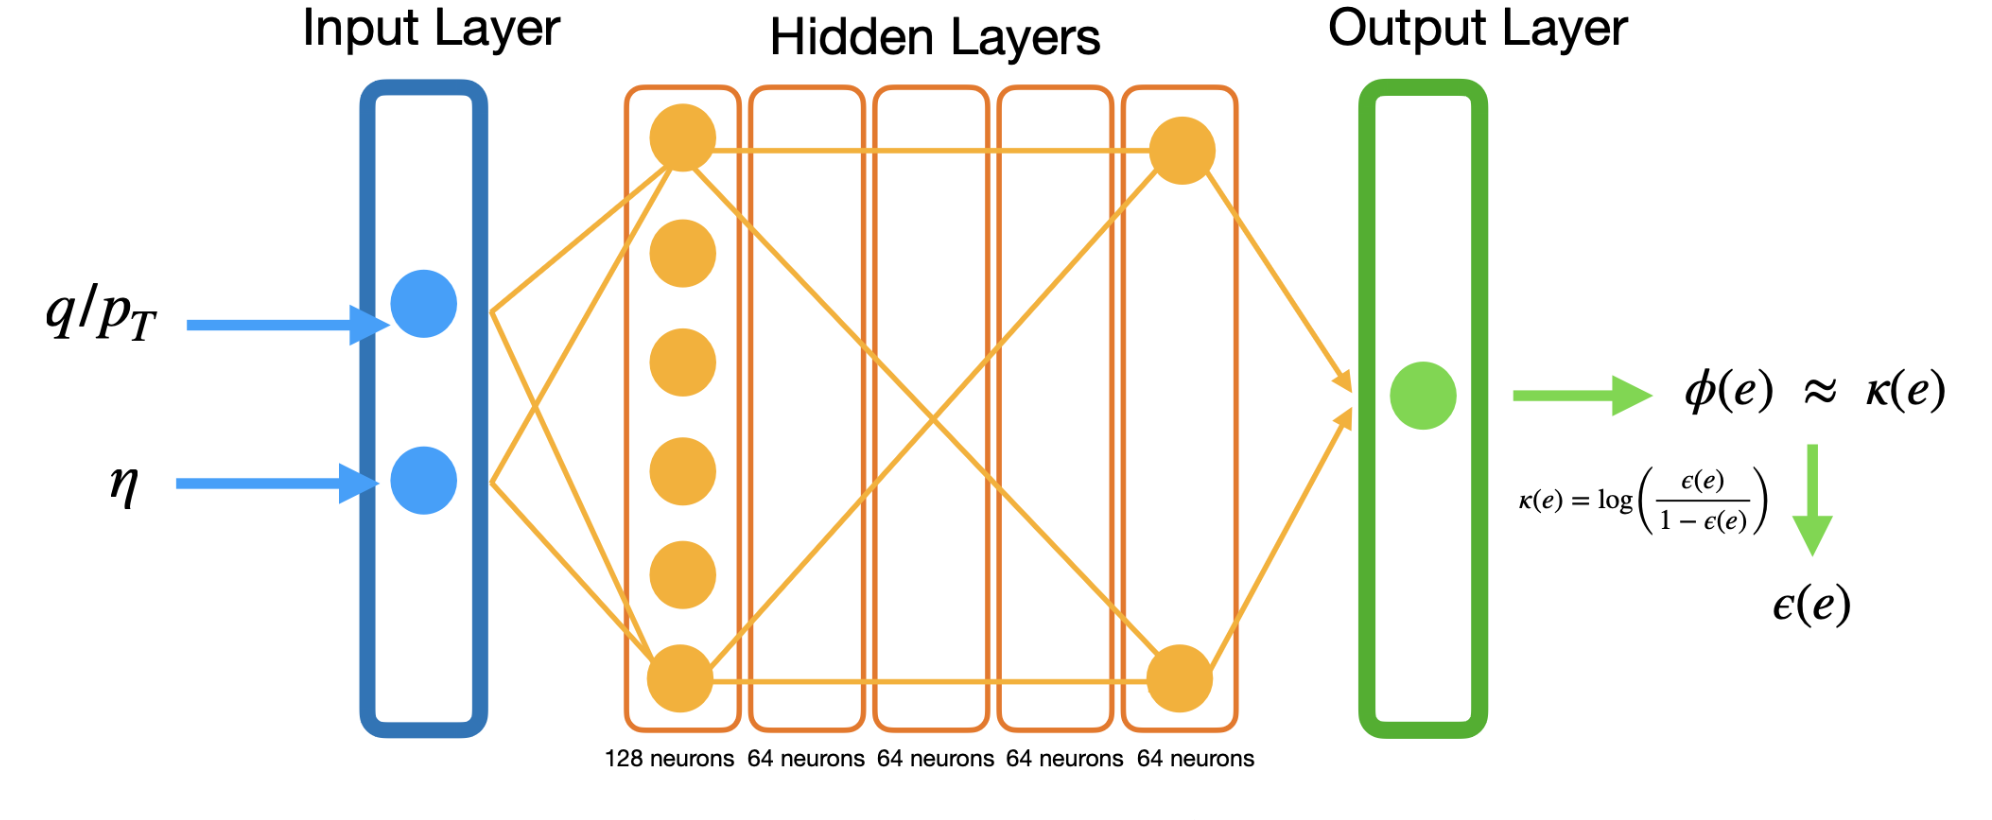
\includegraphics[width=\linewidth]{figures/NN.png}
    \caption{Neural network architecture.}
    \label{fig:nn_arch}
\end{figure}

For the task at hand, the network learns a continuous mapping
\(
\mathbb{R}^2\rightarrow\mathbb{R},
\)
using five hidden layers and producing a single scalar output \(\phi(x)\). This output is inverted to recover the corresponding charge-flip probability  \(\epsilon(x)\). Despite the simple architecture, the network is sufficiently expressive to model the smooth kinematic dependence of charged particle misidentification rates across detector phase space.


\section{Control Region Selection and Object Definitions}

QmisID is estimated in the $Z$-peak region, defined by the di-lepton invariant mass window $81 < m_{\ell\ell} < 101$~GeV, where the standard-model opposite-charge $Z\to ee$ signature is overwhelmingly dominant. Training samples (data and Monte Carlo) are extracted within the QmisID control region, which is constructed to be orthogonal to the 2$\ell$SC signal region. Orthogonality is enforced by the $N_{\text{jet}} < 2$ requirement, highlighted in blue, ensuring the training does not overfit to signal-region characteristics prior to un-blinding. 
\begin{table}[H]
\centering
\caption{Signal region (left) and QmisID control region (right) selection criteria for the $2\ell$SC channel.}
\label{tab:sr_cr}
\begin{minipage}[t]{0.48\textwidth}
\centering
\begin{tabular}{ll}
\hline
\textbf{Selection} & \textbf{Requirement} \\
\hline
Leptons              & Two same-sign leptons \\
Lepton $p_{\text{T}}$ & $\geq 20~\text{GeV}$ \\
Jet multiplicity     & \textcolor{blue}{$N_{\text{jets}} \geq 2$} \\
$b$-jet multiplicity & $N_{b\text{-jets}} = 0$ \\
Dilepton mass        & $m_{\ell\ell} > 12~\text{GeV}$ \\
\hline
\end{tabular}
\subcaption{Signal region}
\label{tab:signal_region}
\end{minipage}
\hfill
\begin{minipage}[t]{0.48\textwidth}
\centering
\begin{tabular}{ll}
\hline
\textbf{Selection} & \textbf{Requirement} \\
\hline
Leptons              & $e^{\pm}e^{\pm}/e^{\mp}e^{\mp}$ \\
Hadronic $\tau$      & $N^{\Sigma Q^{f}}_{\tau_{\text{had}}} = 0$ \\
Jet multiplicity     & \textcolor{blue}{$N_{\text{jets}} < 2$} \\
$b$-jet multiplicity & $N_{b\text{-jets}} = 0$ \\
$m_{\ell\ell}$ [GeV] & $[81,\,101]$ \\
\hline
\end{tabular}
\subcaption{QmisID control region}
\label{tab:qmisid_cr}
\end{minipage}
\end{table}

Electrons are reconstructed by matching energy deposits in the EM calorimeter to tracks in the inner detector. Geometric cuts on both the transverse impact parameter significance $d_0/\sigma_{d_0}$ and the longitudinal impact parameter $z_0$ are made to make sure that electrons originate from a primary interaction vertex. Isolation from other objects is enforced through the lepton isolation working point \texttt{PLV Loose} algorithm.

Jets are reconstructed with the anti-$k_t$ algorithm~\cite{cacciari2008antikt} using a radius parameter $\Delta R = 0.4$, where $\Delta R \equiv \sqrt{(\Delta\eta)^2 + (\Delta\phi)^2}$ denotes the angular separation in the pseudorapidity--azimuth plane. The \texttt{LooseBad} cleaning working point, recommended by the Jet/$E_{\text{T}}^{\text{miss}}$ Combined Performance Group~\cite{atlas_twiki_jetetmiss}, is applied as the default ATLAS jet-quality selection and rejects approximately 99.5\% of fake jets.
\section{Benchmark}
\label{sec:benchmark}

We introduce a benchmark used for training the network. 

\section{Open Data}
\label{sec:Opendata}



\printbibliography

\end{document}
